
\title {The Mainz Endpoint-Tagger}

\section{Motivation}

The Glasow photon tagging spectrometer at Mainz has
an electron band width of 6 to 95 \% of the incoming electron
Energy, $E_0$ \cite{glatag}. After an upgrade \cite{taggup} to accomodate the
energies avaible with MAMI-C, roughly up to 1.6 GeV \cite{mamic}, this will
allow for tagged photon energies up to roughly 1.54 GeV. In order to
increase this photon energy, post bremsstrahlung electrons of energies
below roughly 100 MeV have to be detected, which is not possible with this
Main Tagger, MT. The goal can be achieved by installing a small tagger
upstrem of the MT, which then detects these lower energy eletrons. It is
reasonable to build this Endpoint Tagger, ET, such that there is an overlap
of the band widths of both taggers, ET and MT. Therefore, the ET should be
capable of detecting post bremsstrahlung electrons with energies up to
at least 150 MeV. When the ET is used, the MT
can only serve as a cleaning magnet. In order to guide the main beam safely to
the electron beam dump an additional Correcting Magnet, CM, is needed that
corrects for the deflection of the main beam by the ET.

Whit this installation in operation it is possible, for example,
to investigate the threshold region for the production of $\eta'$ mesons.

Since adding ET and CM to the tagger set-up will only be needed for special
experiments, this addition will be built such that it can take the space
which otherwise a goniometer box has, which helps to privide linearly
polarized photons from coherent bremsstrahlung. Thus, these two installations
can be interchanged.


\section{The ET-CM-MT set-up}

Figure \ref{etcmmt} shows the set-up of the magnets ET, CM and MT
in its location in the MAMI tagger-hall.\\

\begin{figure}
%\vspace*{-1cm}
\begin{center}
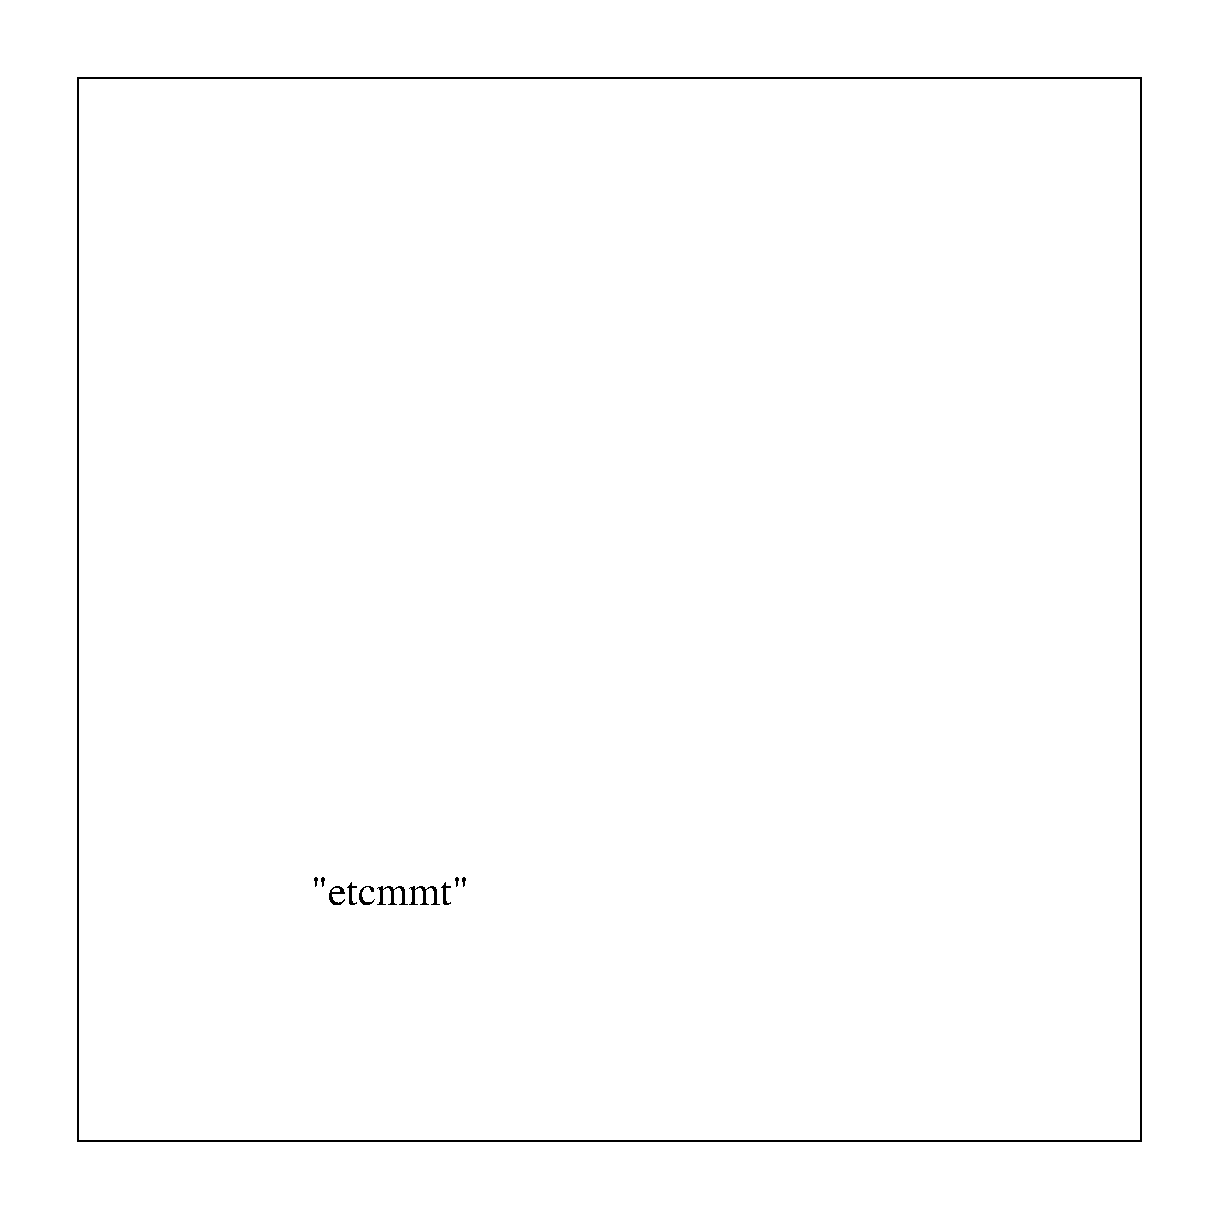
\includegraphics[height=8cm]{./et_etcmmt.eps}
\vspace*{-1cm}
\end{center}
\caption{The Glasgow photon tagger, MT, complemented by an endponit
tagger, ET, and a correction magnet, CM. Only the main beam is indicated,
which ends in the beam dump, BD}
\label{etcmmt}
\end{figure}

The magnets ET and CM had once been used in the low-energy
Glasgow Tagger \cite{lowglatag} and there were named DS2 and DS4.
Modofications were needed in order to serve
the present purpose. In ET the Rogowski profiles were filled in with iron
and the pole gap was reduced from 8\,cm to 2\,cm by inserting two iron
plates which then also serve as top and bottom of the vacuum chamber.
Similar changes were made to turn DS4 into the correctionmagnet, CM. 
As a result fields up to 1.4\,T can now be generated in ET.

\section{The endpoit tagger, ET}

Figure \ref{map14} shows a field map of ET as measured with a current of
300\,A (???). \\
\begin{figure}
%\vspace*{-1cm}
\begin{center}
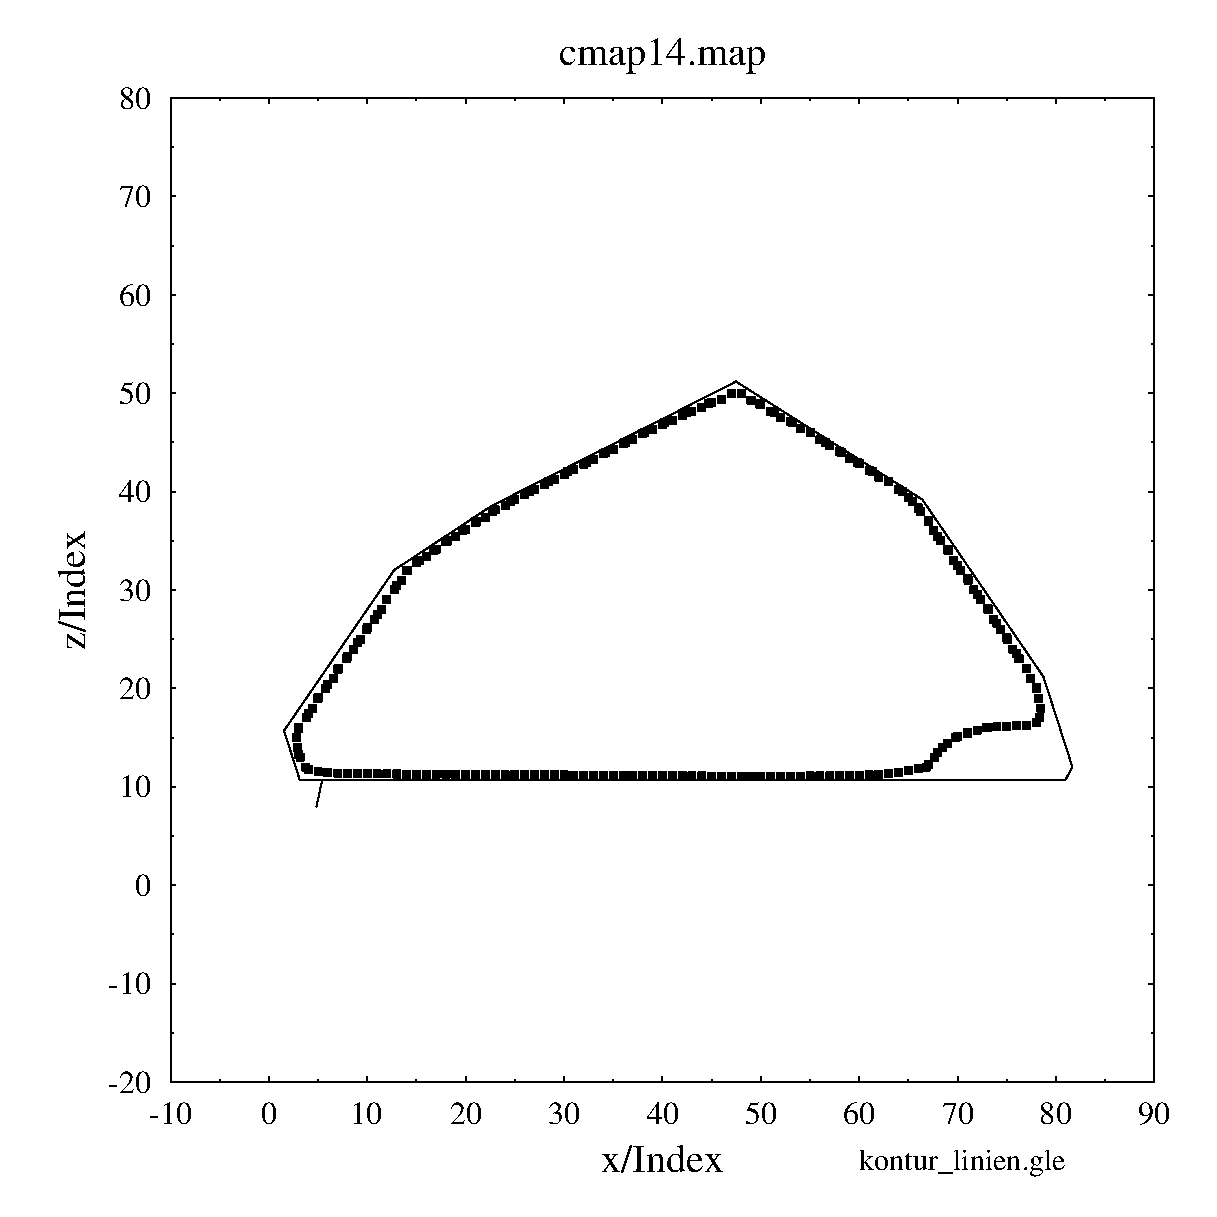
\includegraphics[height=8cm]{./et_map14.eps}
\vspace*{-1cm}
\end{center}
\caption[*]{Field map in ET measured with a current of 300\,A (???),
shown are different lines of costant magnetic field.}
\label{map14}
\end{figure}
This field map was then taken to raytrace electrons of several energies
through the magnet from which the point to point focus of the 
radiator is obtained,
as shown in fig. \ref{trajet}.

\begin{figure}
%\vspace*{-1cm}
\begin{center}
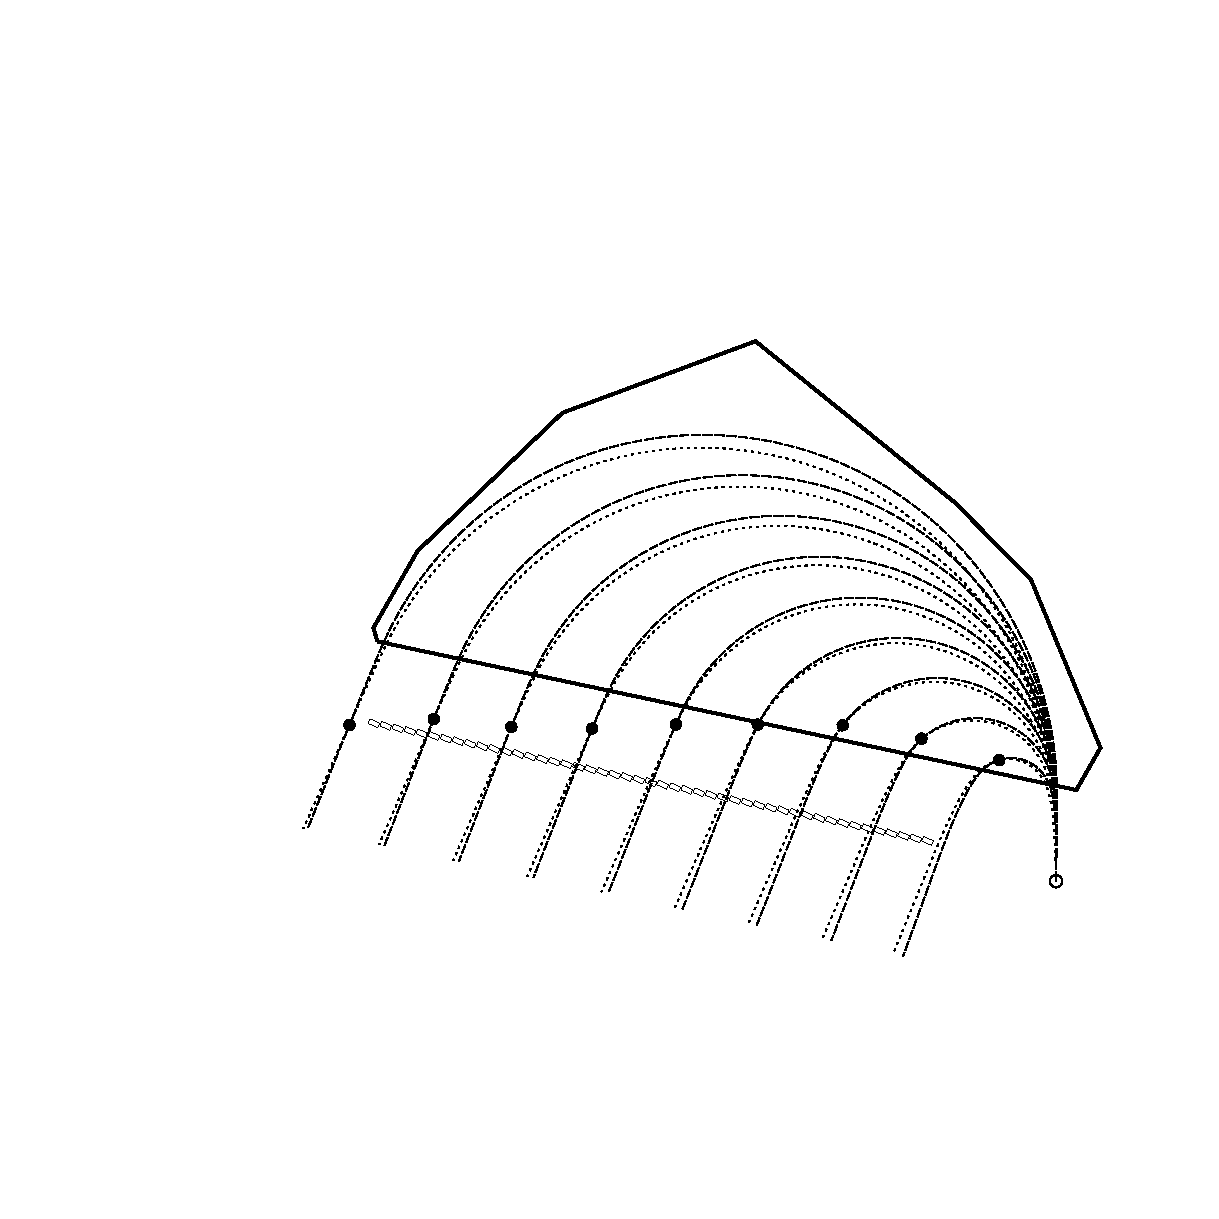
\includegraphics[height=8cm]{./et_raytrace.eps}
\vspace*{-1cm}
\end{center}
\caption{Electron trajectories in ET for energies 20 to 160\,MeV in 
steps of 20\,MeV, starting at angles $\pm$1$^o$. Magnetic field 1\,T.
The solid lign gives the dimension of the poleface. 
The circle indicares the positin of the 
radiator, the dots give the point to point focus. 
The detectors are shown as rectangles (length of the ladder **cm).}
\label{trajet}
\end{figure}

The low energy part of the focus line is inside the gap of the 
magnet, which is not convenient for mounting the electron detectors.
Thus it was decided to install the tagger detector ladder outside the magnet
coils. This position is indicated in the figure.
By doing this, part of the resolution of the tagger is sacrificed, especially 
for low energy electrons. Figure \ref{resolution} depicts the resolution
found along the point to point line and along the chosen line as well as 
the dispersion found for both cases.\\

\begin{figure}
%\vspace*{-1cm}
\begin{center}
\includegraphics[height=8cm]{./et_res_dis.eps}
\vspace*{-1cm}
\end{center}
\caption{Resolution and dispersion for post-bremsstarhlung electrons
up to 170 MeV (1.4 T in the gap). Both properties are shown for the ideal case, 
along the point to point line, and the realistic case.}
\label{resolution}
\end{figure}

According to this result, the detectors were chosen to be equally spaced
by 14\,mm (????)
and 13\,mm wide. A total of 47 detectors is used.
The detectors are not overlapping. 
Each single tetector is a unit and thus can be exchanged without influencing 
the rest of the detector-ladder.
They are 6\,mm thick, which gives good signals and allows for
calibration with an ??? electron source, by chosing coincidence signals with
an equal detector behind the scintillator to be investigated.
Due to strong stray filds of the magnet, long light guides had to be used.

Figure \ref{detector} shows a drawing of the detector and the final
set up of the detector ladder.

\begin{figure}
%\vspace*{-1cm}
\begin{center}
\includegraphics[height=8cm]{./et_detector.eps}
\vspace*{-1cm}
\end{center}
\caption{********}
\label{etector}
\end{figure}


\begin{thebibliography}{99}
\bibitem{mamic} MAMIC
\bibitem{glatag} Glasgow-Tagger
\bibitem{taggup} upgrade of GT
\bibitem{lowglatag} low energy GT


\end{thebibliography}
